\chapter {Иорданский ручей}

Об Иорданском ручье сведения неясны. 

На нескольких картах 19 и 20 веков отмечен, однако не подписан, ручей, берущий начало в глубине существовавшего тогда оврага по Мыльному переулку, и продолжающийся на северо-восток в сторону Чернечьего или Черного («старого» Иорданского) озера, подробнее о котором сказано в главе про Почайну.

Киевские диггеры называют Иорданским ручей, что начинается приблизительно от источника на территории новой, построенной в котловине бывшего глиняного карьера, Никольско-Иорданской церкви, текущий в трубе под Мыльным переулком и далее под улицей Заводской в сторону Гавани, очень вероятно повторяя путь ручья, упомянутого абзацем выше.

Я хочу разобраться, что называли Иорданским ручьем в 19 веке. Разобраться трудно, ибо прошло много времени и местность изменилась. Как вообще работает родник в склоне горы, или, говоря языком геологии, пластовый источник? 

Гора состоит из слоев грунта. Осадки впитываются в эти слои до некоего нижнего слоя, который не пропускает воду. Это может быть, например, слой глины, которая, намокая, перестает проводить воду. Слои, копящие в себе воду, называются водоносным горизонтом. Если водонепроницаемый слой имеет уклон в сторону склона, то вода из горизонта начинает туда двигаться и выходить на поверхность в виде родника.

Водонепроницаемый слой может быть на уровне середины горы, или внизу – как получится. А чем больше площадь водоносного горизонта и его толщина, тем больше он может впитать воды и снабжать ею источник, если, конечно, сам горизонт в свою очередь получает питание от осадков.

Склоны же Лысой горы и окрестностей столь великое множество раз перекапывались и уничтожались, что водоносный горизонт и водонепроницаемый слой многократно изменялись. Значит, выходы родников из склона могли смещаться, и сейчас пожалуй нельзя восстановить историю здешней природной водной системы.
 
Как мы знаем со слов Похилевича, близ Иорданской церкви было нечто вроде колодца, куда поступала вода по трубам из другого колодца, на уступе горы, выше церковного погоста. Этот нижний колодец и слыл чудодейственным Иорданским источником. Поскольку современная Иорданская церковь находится на другом месте, чем прежняя, то современный источник, откуда берут воду прихожане – вероятно тоже в другом месте.

Возникает несколько вопросов относительно положения дел в 19 веке. Имеет ли отношение ручей, протекавший в Мыльном переулке, к легендарному источнику?

Вспомним сообщение Лохвицкого, где он пишет сначала об остатках, как он полагает, древней Ильинской церкви: 

\begin{quotation}
Место сей церкви и остатки фундаментов
каменных, отрытых из недр земли при изследовании Лохвицким, находится на выезде из Киева в Кирилловское богоугодное заведение,
за Иорданскою церковью, от дороги по левой
стороне, повыше бывшей Богословской церкви,
в полгоры над ручьем так называемым Иордан-
ским.
\end{quotation}

Если «повыше бывшей Богословской церкви», а не Иорданской церкви, то получается мыс с «Кожевником». Ручьи есть и были по обе стороны этого мыса.

Но!

\begin{quotation}
Ручей Иорданский пониже и подле сего места течет, а вытекает повыше, с горы, близ сих остатков Ильинской церкви. Сей ручей начало берет из ключей железистых, которые приметны по ржавчине железной в источнике родника сих ключей.
\end{quotation}

Раз ручей Иорданский, то он должен быть и неподалеку от Иорданской церкви, а не по другую сторону мыса «Кожевника». Логика приводит нас к оврагу между «Кожевником» и соседним мысом Лысой горы, оврагу с дорогой, что Похилевич именовал «Никольским старым ввозом» и древней дорогой на Лукьяновку. И да, там протекает ручей, ныне в коллекторе.

Когда я там лазал, то не был знаком с сообщением Лохвицкого, и поиски ручья вел несколько северо-западнее.

По нижней половине склона от Богуславского спуска до Иорданского переулка (на современных картах его обозначают тоже Мыльным), под горой с дачами «Кожевника», не достигая долготы нотной фабрики, есть дренажная система, местами доступная для просмотра. В бетонных комнатках видны толстые керамические трубы и течение воды. Уже над фабрикой молочной кислоты, в одном из открытых узлов системы просматривается труба откуда-то сверху, со стороны «древней дороги на Лукьяновку». В зарослях ближе к оврагу с этой дорогой, прямо из горы сочится бурый родник, увлажняя смешанную с грязью траву и листья.

Лохвицкий говорил, что ручей Иорданский составлялся из нескольких, именно нескольких «ключей железистых». Родники, сливаясь, и давали более ощутимый, чем по отдельности, поток.

Вот несколько снимков 2013 года с задворков фабрики молочной кислоты.

Сначала – колодец захвата грунтовых вод, оттуда труба ведет примерно на, как я помню, юго-восток:

\begin{center}
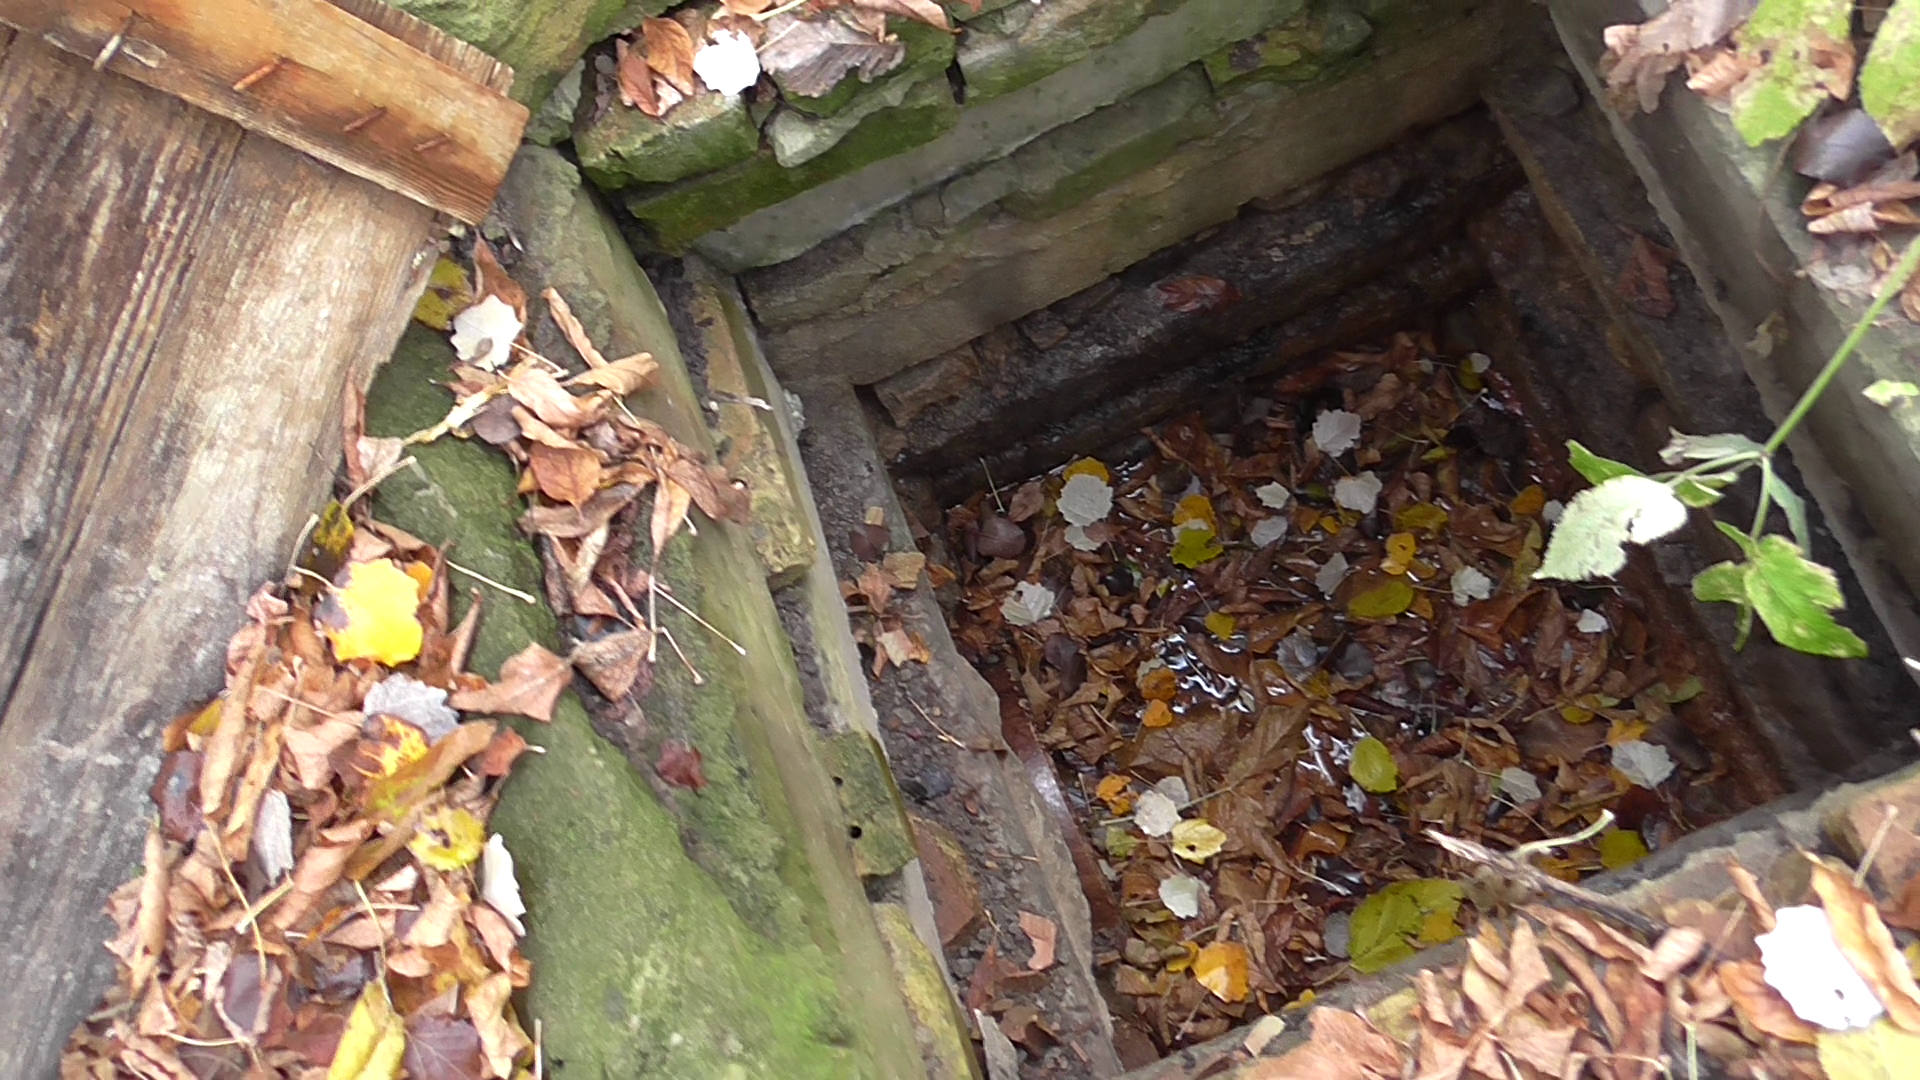
\includegraphics[width=\linewidth]{chast-kirvys/iordanruch/s_vlcsnap-2014-05-16-20h08m14s138.jpg}
\end{center}

А вот место, где собирается вода из двух труб и направляется в трубу на северо-восток, в направлении фабрики молочной кислоты и улицы Кирилловской. Рыжее на снимке и есть признак «железистости». Её можно наблюдать на родниках из склонов озера Глинки, а также в ручьях Репяхового и Бабьего яров.

\begin{center}
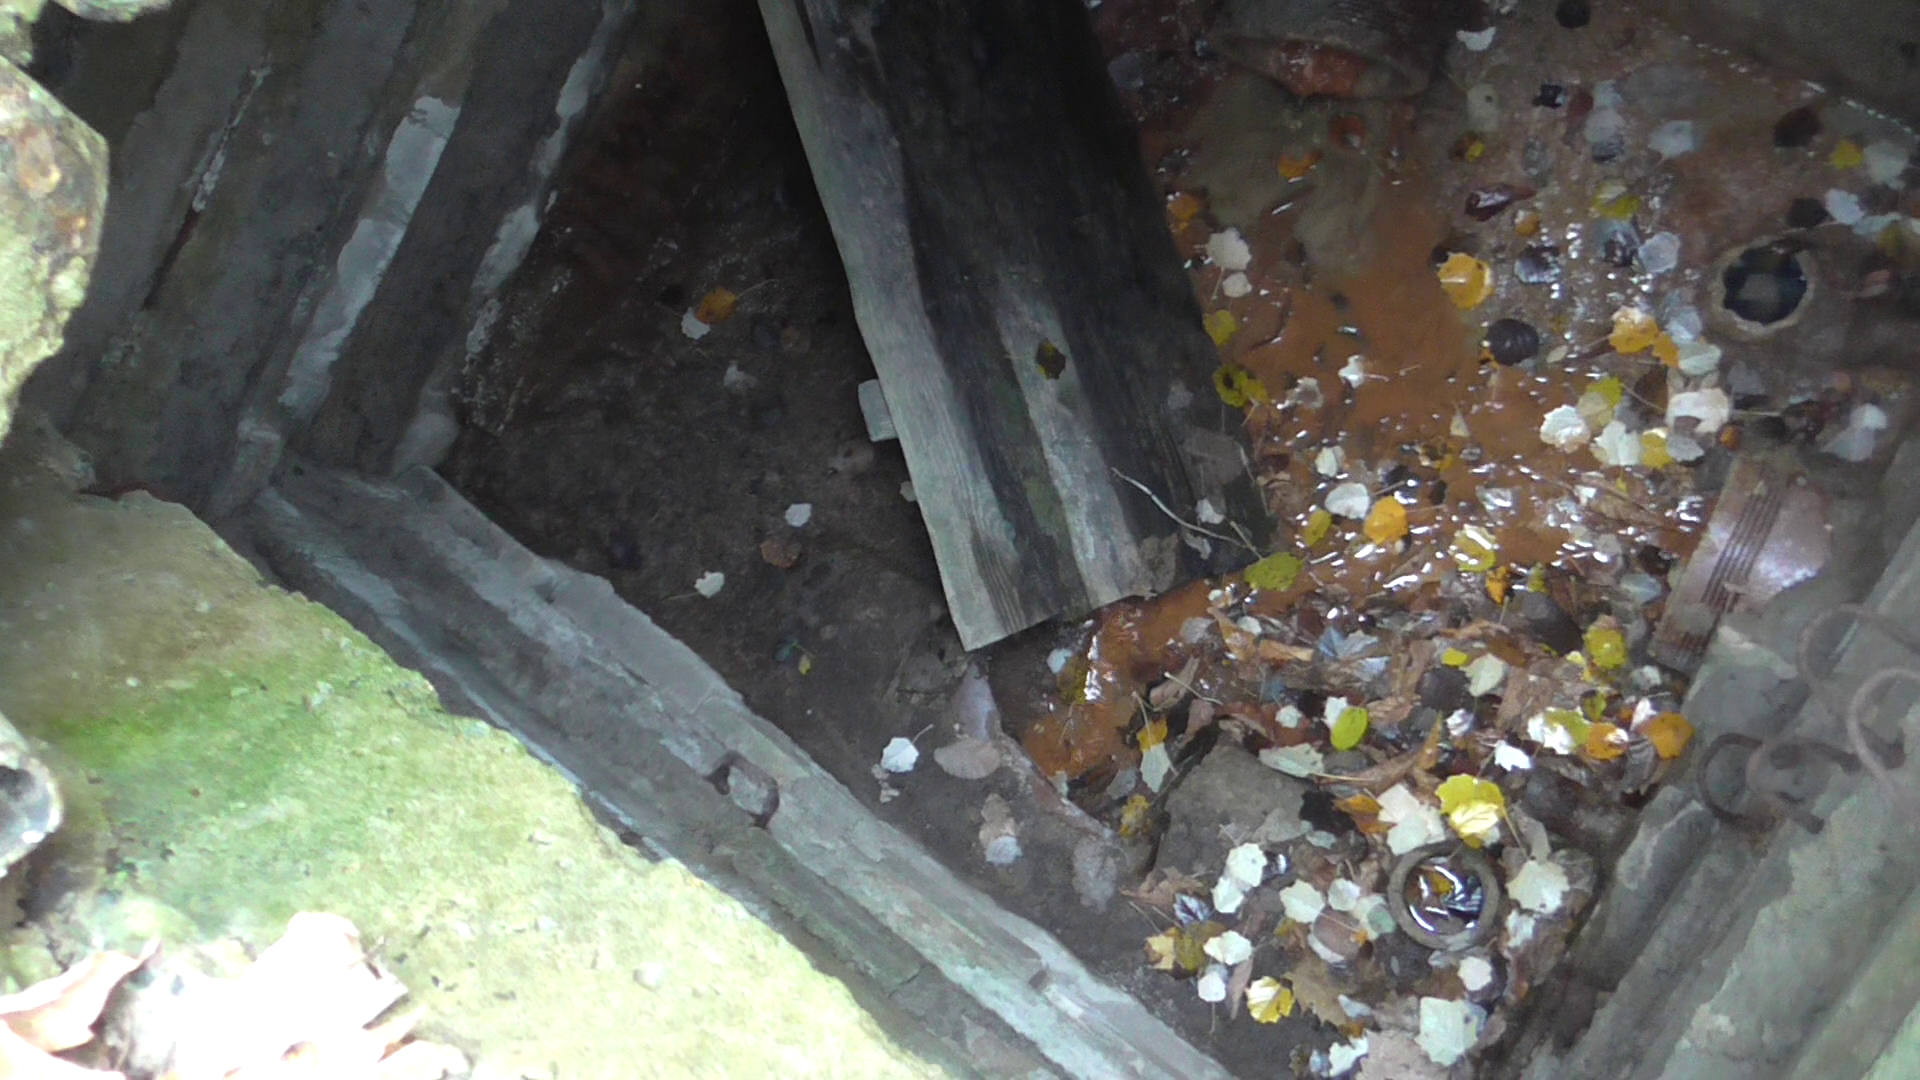
\includegraphics[width=\linewidth]{chast-kirvys/iordanruch/s_vlcsnap-2014-05-16-20h10m19s241.jpg}
\end{center}

Что же, Иорданский ручей начинался над нынешней фабрикой молочной кислоты? Из склона под «Кожевником» в том числе, а также выше по оврагу «Никольского старого ввоза».

Добавим доказательств.

Вот источник редкий, приведу его полностью. План Иорданского монастыря за 1835 год, со всеми его строениями. Легенду карты (с ошибками подлинника, но частичным приведением к современному написанию) даю текстом, а сам план – фотокопией.

\begin{center}
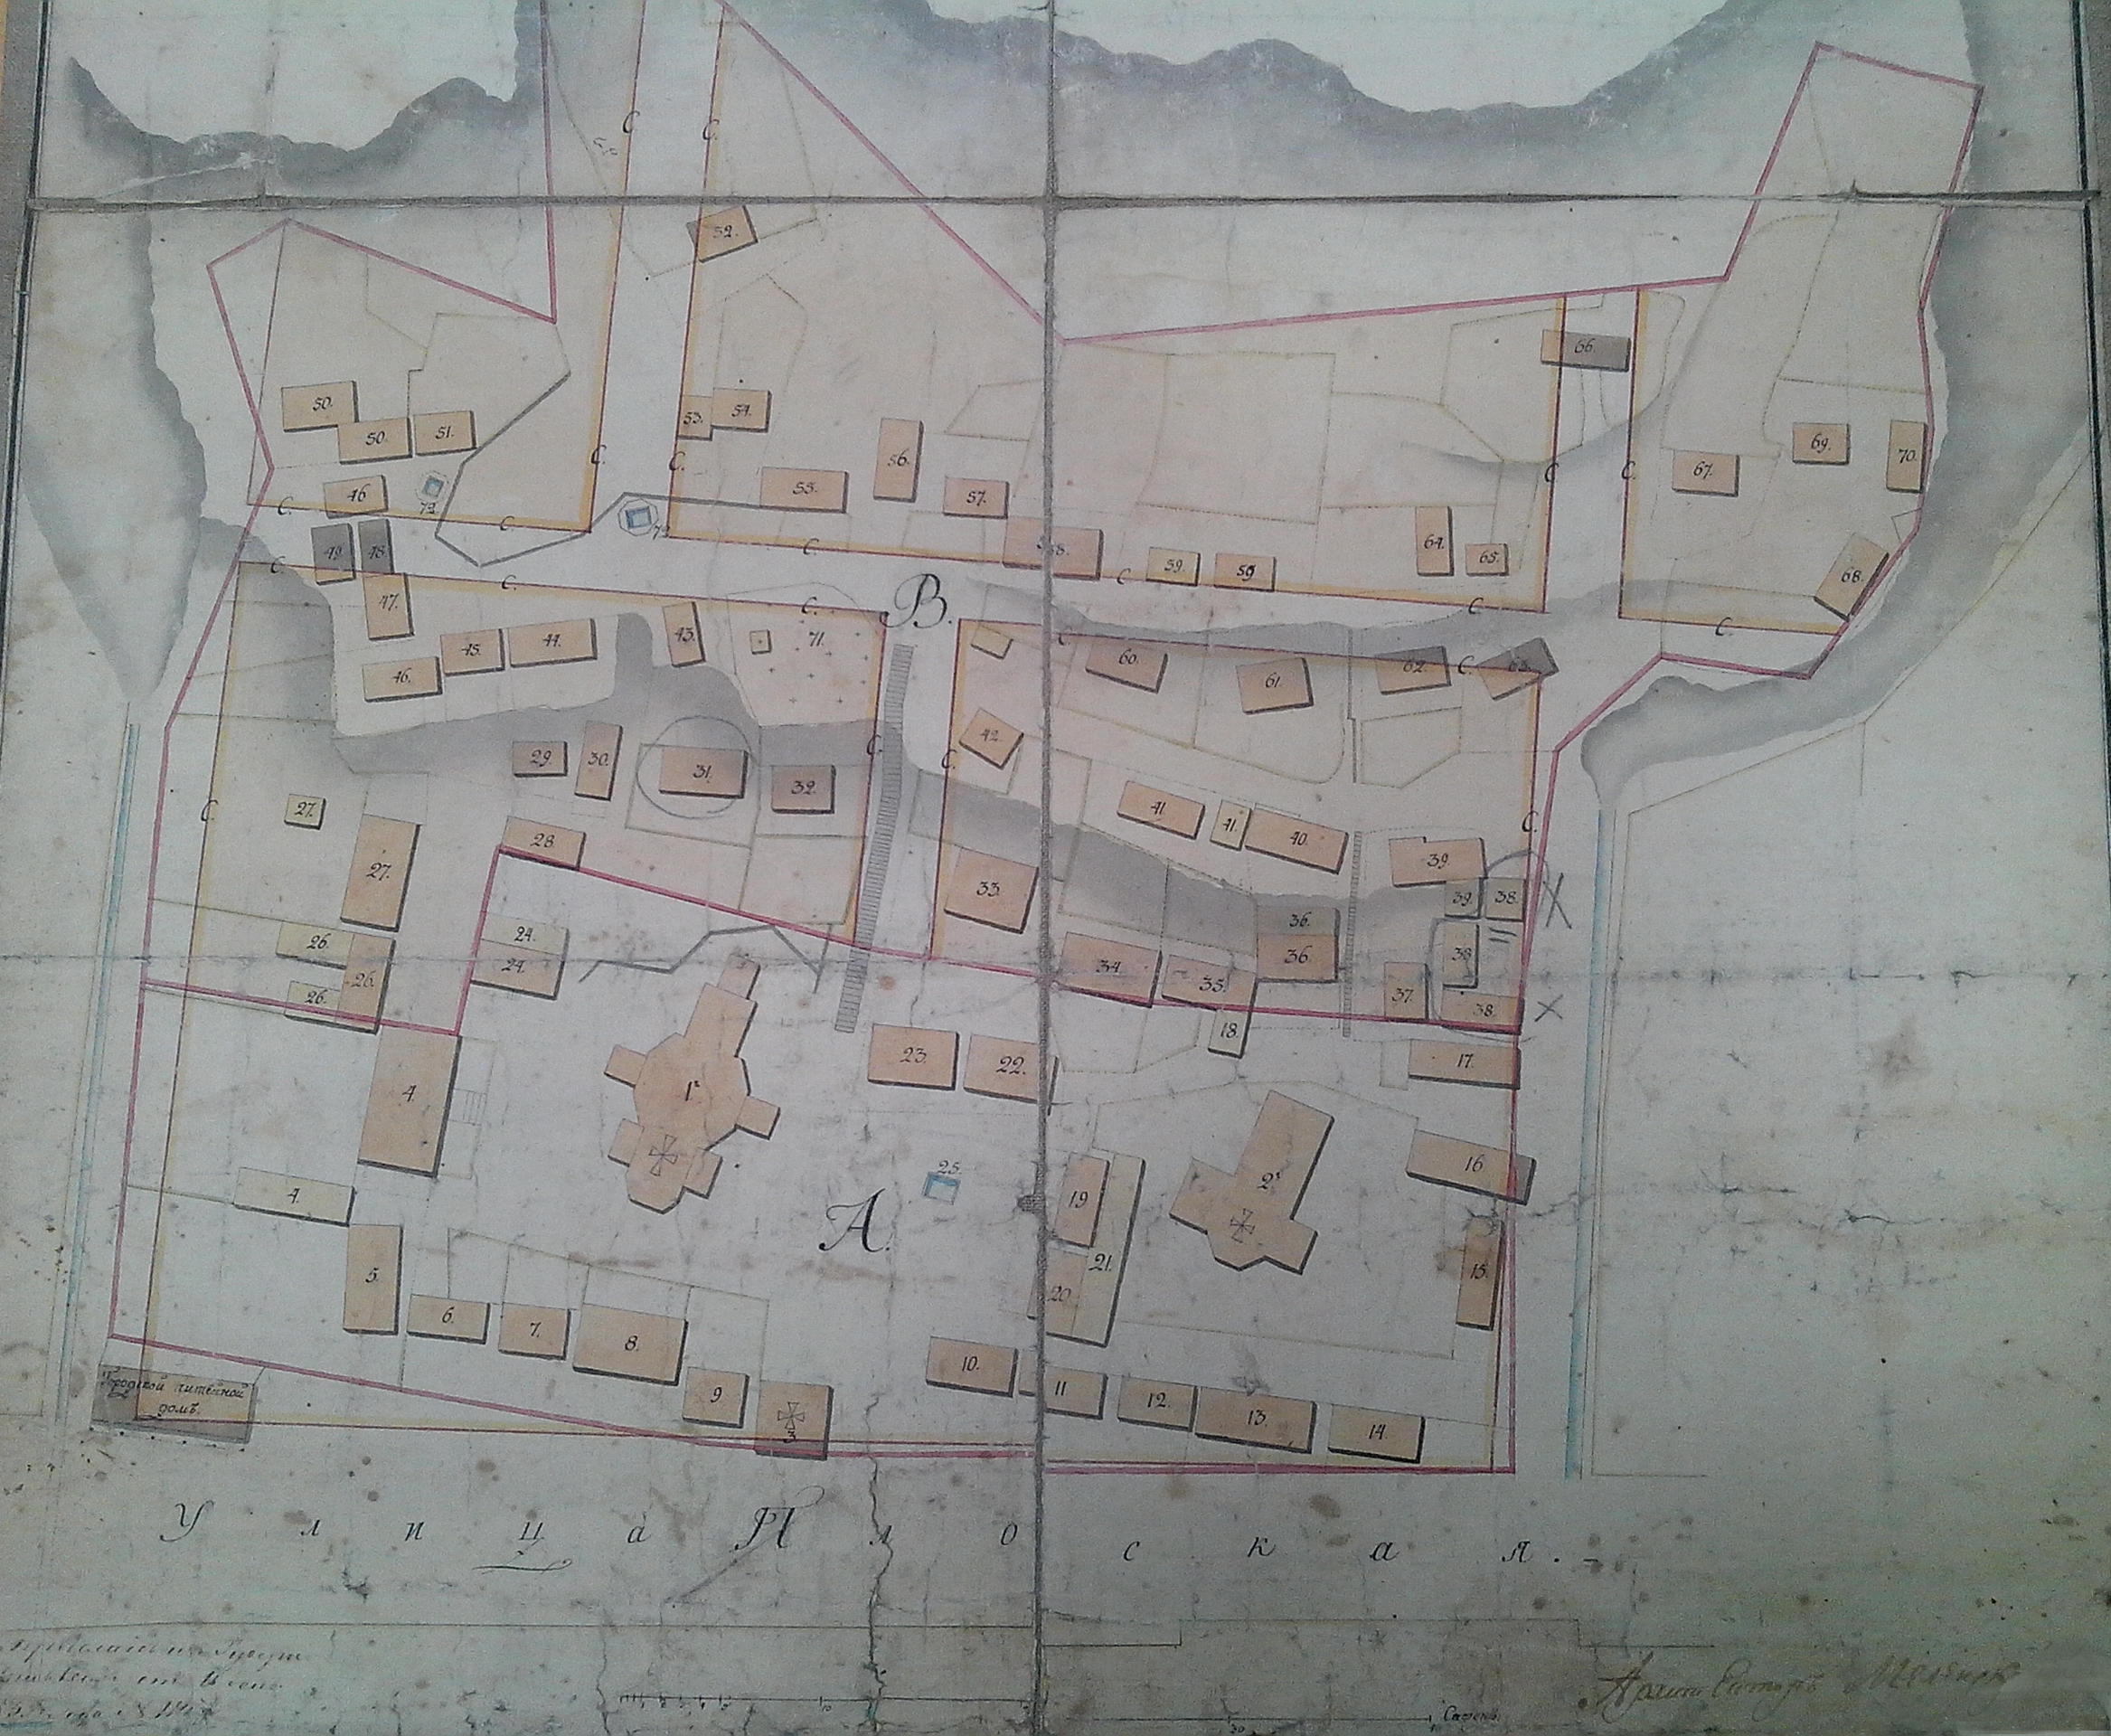
\includegraphics[width=\linewidth]{chast-kirvys/iordanruch/IMG_20170627_142118.jpg}
\end{center}

План местоположению упраздненного Иорданского женского монастыря, снятому по Указу киевского губернаторского правления состоящему в ? части города Киева на Плоском, который назначен в обращение в приходскую церковь, с показанием на сем плане числа квадратных сажень исчисленных, по примерному назначению пространства для церковного погоста и в остающейся части занимаемой под заселение онаго монастыря, что означенно красными линиями, с объяснением кому именно находящиеся на нем деревянные кельи и строения ныне принадлежат.

\newpage

ОБЪЯСНЕНИЕ ПЛАНА

А: Место примерно назначаемое для церковного погоста, Заключающее пространства тысячу шесть сот семдесят пять с одною третью квадратных сажень; на коем находятся деревянные строения именно:

1. Церковь во имя святителя и Чудотворца Николая.

2. Теплая церковь во имя святителя Димитрия Мироточца.

3. Колокольня. 

4. Корпус начальничьих келий и сараи.

5. Келья девицы Евдокии Бриенковой.

6. Монахини Надежды.

7. Монахини Евсесии.

8. Монахини Елены и вдовы дияконихи Марины Дьяковской.

9. Монахини Калиствены Степиодоты.

10. Монахини Порьфирии.

11. Манахини Евлампии.

12. Монахини Мокрины.

13. Вдовы священнической жены Евдокии.

14. Монахини Евгении.

15. Вдовы подпорутчицы Евдокиии Тюриковои и девицы Агафии Гриневичевой.

16. Монахини Спеклитикии.

17. Девицы Ефимии Димченковои.

18. Небольшой анбарчик вдов Ефросинии Дьяченковои и Устины Котлярки, и девицы Настасьи Шевченковои, коих келья за границею погоста.

19. Прежде бывшая келья монахинь Мамельхи и Серафимы, а ныне купленны Церьквою.

20. Монахини Палагеи.

21. Церковнои сараи.

22. Монахини Смарагды.

23. Вдовы священнической жены Ксении Бурмовской и монахини Нектарии.

24 Келья и сарай вдовы придворного Ганнимебера Феодосиии Петровой.

25. Колодец.

В: За исключением погоста остающаяся часть оного монастиря заключающая пространства три тысячи триста девятдесят и две три квадратных сажень, на которой находятся деревянные строения именно:

26. Келья и два сарая Скимонахини ксении.

27. Келья и погреб молдавской монахини Александры.

28. Молдавских монахинь Феофанны и Павлины.

29. Мещанки вдовы Елены Крамаренковой.

30. Девицы Акилины Петровой.

31. бывшая келья мещанки Анны Морозовой, а ныне мещанина Герасима Ермаченко.

32. Девицы Евдокии Герасимовой и вдовы Евдокии Корнилиевой.

33. Монахини Павлы.

34. Монахини Мокрыны.

35. Вдовы Ефросинии Дьяченковой и Устины Котлярки и Девицы Настасии Шевченковой.

36. Келья и сарай бывшие монахини Александры, а ныне вдовы Анны Морозовой.

37. Келья бывшая монахини Анфии а ныне мещанина Зеновия Савченка.

38. Келья, коморка и сараи бывшие монахинь Проклы и Палладии, а ныне мещанина Козьмы Шевченка.

39. Келья и сараи девицы Дарьи Буровой.

40. Бывшая монахини Марьяны, а ныне мещанки вдовы Евдокии Скляревской.

41. Келья и сараи Сержантши Домны Савельевой.

42. Солдатки вдовы Татьяны Фоминцовой.

43. Келья бывшая монахини Арсавии, а ныне пономаря Никиты Гилевича.

44. Мещанок вдов Ульяны Котляровой и Устины Михаревой.

45. Вдовы Губернской секретарши Евдокии Гриневской.

46. Две кельи девицы Прасковьи Синютиной.

47. Вдовы Ксении Штанькевички.

48. Бывшая келья монахини Евсевии а ныне а ныне мещанина Ивана Головаченка.

49. Солдата Яковлева.

50. Две кельи девицы Марфы Андреевой.

51. Вдовы Анны Марченковой.

52. Девицы Натальи Воиновой.

53. Вдовы Анны Садововны.

54. Вдовы солдатки Степаниды Лебедевой.

55. Девицы Меланьи Девятисиловны.

56. Девицы Ефимии Батяниной.

57. Девицы Настасии Дичинской.

58. Мещанки вдовы Аксиньи Корчинской.

59. Келья и анбар вдовы Кронтшадского Гезеля Ульяны Ушаковой.

60. Мещанки Екатерины.

61. Девицы Екатерины Жидовозновны.

62. Вдовы Козачки жены Екатерины Крымченковой.

63. Девиц Варвары и Ирины Лупичевских.

64. Девицы Агафии Степуровны.

65. Вдовы Евдокии Федоровой.

66. Девицы Харитины и вдовы Агафии Ромурки.

67. Девицы Домникии Ванфевны.

68. Вдовы Попадьи Анны.

69. Принадлежащая келья монахини Елены.

70. Вдовы салдатки Февроньи Шевелевой и вдовы мещанки Марины Лозовской.

71. Кладбище.

72. Два Колодца.

С. в оной остающейся части монастыря наложенной проекте вновь улицам с означением кварталов под желтою краскою, и что отходит под те улицы в сломку покрыто жидкою тушью.

Эта карта – своего рода ребус, который нельзя решить, не зная, как изменялась местность. Мы решим только одну загадку.

Вот сейчас у нас есть часть современного Мыльного переулка, что лежит параллельно Кирилловской улице\footnote{Ранее этот отрезок слыл частью Иорданского переулка.}. На плане 1835 года примерно там проходит дорога с большой буквой В, к которой снизу подходит нечто вроде лесенки.

И внизу церковной усадьбы у нас улица Плоская, ныне Кирилловская.

Участок между Кирилловской и тем отрезком Мыльного сейчас плавно повышается в сторону двух больших мысов. Но раньше, как видно на плане 1837 года, там был еще один уступ горы, начинавшийся прямо над обеими церквями. То бишь домики на плане 1835 года, изображенные выше церквей, на самом деле стоят на пригорке относительно церквей.

Таким образом кладбище, обозначенное номером 71, было на этом уступе, в районе «параллельного Мыльного». Это не одно из тех кладбищ, что были еще выше на мысах «Кожевника» и Лысой горы. Это третье, малое, не сохранилось ни в коей мере, как и на «Кожевнике».

Вопрос колодцев с этим знанием рельефа решается просто. Похилевич в 1865 году упомянул о:

\begin{quotation}
монастырском колодце, существующем и ныне на уступе горы, выше нынешнего церковного погоста, из которого проведена трубами превосходная вода в нижний, близ нынешней церкви.
\end{quotation}

На карте 1835 года мы видим рядом с буквой «А» колодец под номером 25, а выше на карте  еще два колодца, слева от буквы «В». В самом деле, эти колодцы (вероятно ко времени Похилевича остался один) находятся выше и погоста, и колодца 25.

Большая Николаевская церковь обозначена номером 1. Как решить ее наличие на карте 1835 года, если сведения Похилевича про пожар 1821-го верны, я не знаю. Поодаль стоит деревянная Дмитриевская церковь, под номером 2, вместо которой потом построили где-то поблизости одноименную каменную. Я не могу соотнести места двух церквей на плане 1835 года с современным рельефом.

Голубые «каналы» по обеим сторонам усадьбы – не пущенные ли по канавам ручьи? Ручей по бывшему Иорданскому переулку и ручей по Мыльному-перпендикулярному Кирилловской?

На плане 1837 года я нашел подробное изображение обоих ручьев!

\begin{center}
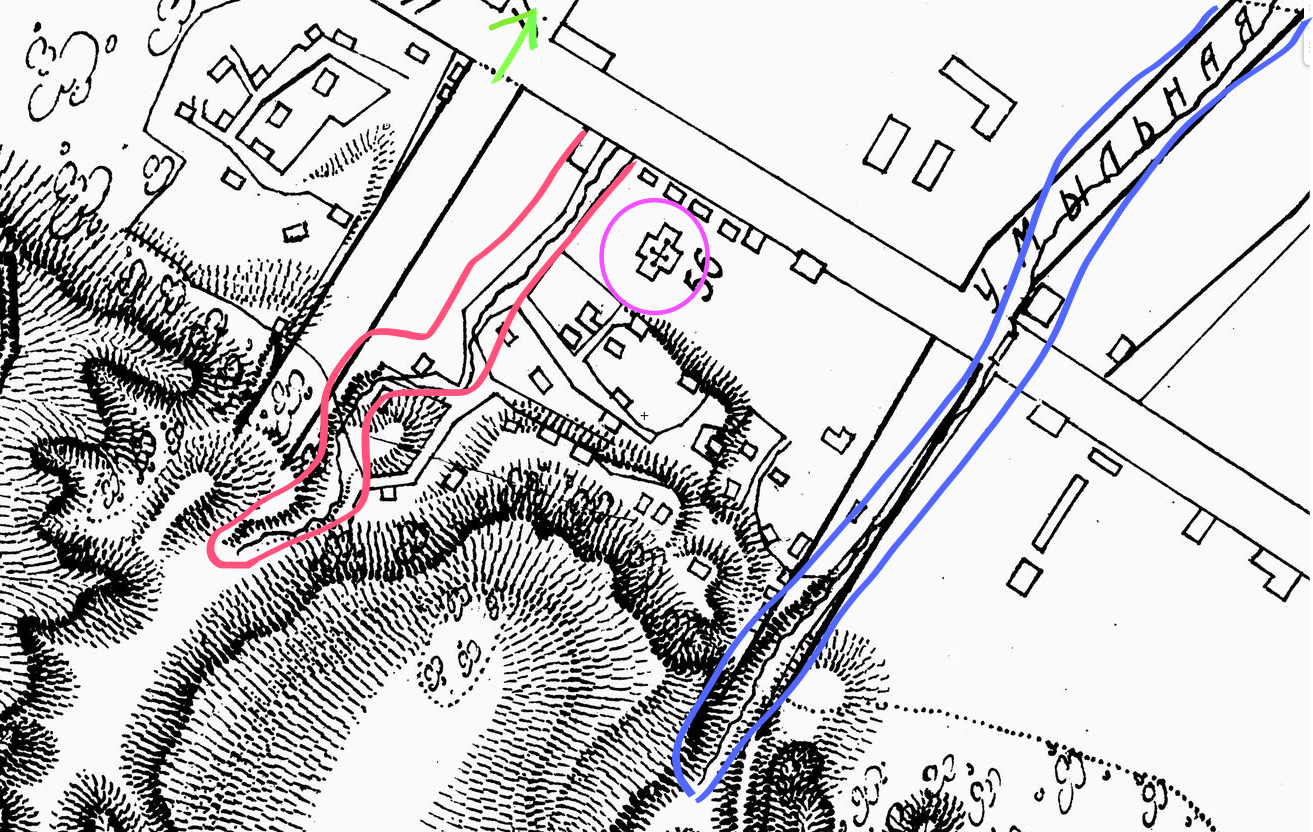
\includegraphics[width=\linewidth]{chast-kirvys/iordanruch/map.png}
\end{center}

Зеленая стрелочка – показана улица Заводская, она и ныне там. Мыльная улица исчезла, ею бы продолжался современный Мыльный переулок. Перпендикулярная ему улица, конечно же, Кирилловская. Синим я отметил ручей, вытекающий – о да – из Мыльного переулка, и при наложении на спутник имеет устье этого ручья точнехонько в источнике близ современной Иорданской церкви-новодела. Этот источник сочится из подножия склона.

Фиолетовым я отметил... А вот где-то там стояли 
обе прежние Иорданские церкви, на плане числом 56 обозначены «Каменная и деревянные приходские церкви», то есть обще и условно. Ниже их видим тот самый уступ горы, который прежде существовал, а ныне отсутствует, сглажен.

Розовым – тот самый ручей, что берет начало на склоне выше старых Иорданских церквей. При наложении на спутник получаем, что он протекал... Вдоль «старого Никольского ввоза», дороги в овраге между мысом Лысой горы и «Кожевником»! А затем по Иорданскому переулку в сторону Кирилловской улицы.

При этом, повторюсь, все задворки церкви (ныне задворки фабрики молочной кислоты), я обвел их желтым, это подножие холма – все они сочатся родниками, взятыми в дренажку, но прежде они тоже куда-то стекали.

Дальнейшее движение «розового» ручья на карте, от Заводской улицы, не показано. Однако именно он подходит под письменные описания Иорданского ручья – начинается на склоне над церковью, в самом деле разделял бы Иорданский и Богословский монастыри (есть сведения из непроверенного мною источника, что Иорданский ручей протекал между Иорданским и Богословским монастырями, разделяя их помимо рукотворной ограды). Поныне, около схода со склона к Иорданскому переулку, по заброшенной лестничке близ развалин старого дома есть остатки коллектора.

Учитывая большую даже сейчас насыщенность там водоносного горизонта и множество родников, полагаю следующее. Иорданский ручей слагался из ручьев между отрогом Лысой горы и мысом дач «Кожевника». Ручей был достаточно велик, чтобы Лохвицкий смог проследить его течение до устья в Иорданское озеро. \textbf{Иорданский ручей протекал через Иорданский переулок и Заводскую улицу}.

\textbf{Другой ручей} протекал через Мыльный переулок (от современной Иорданской церкви) и совпадает с «диггерским» Иорданским ручьем.

\begin{center}
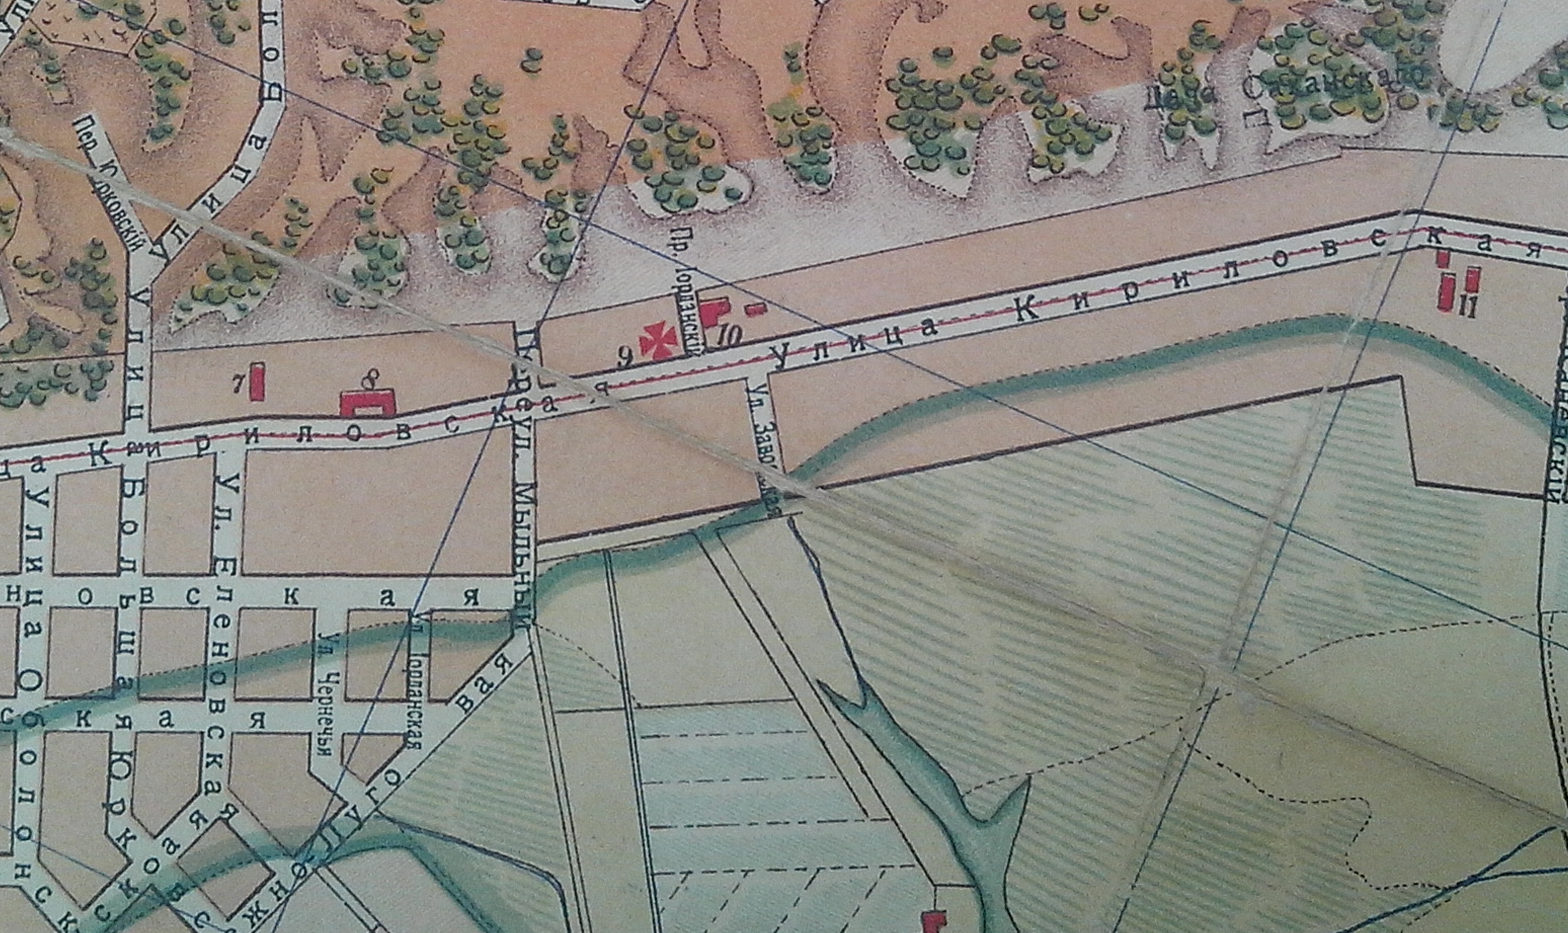
\includegraphics[width=\linewidth]{chast-kirvys/iordanruch/map-1903.jpg}\\

Кусок плана 1903 года.
\end{center}

На планах 19 и начала 20 веков, рисуют, но не подписывают, то ручей из Мыльного переулка, то ручей из Иорданского переулка. 

Доселе я не касался разбора названия Иорданского монастыря, приводя лишь расхожую легенду о чудесном источнике, где всплыл ковшик, оброненный паломником в Палестине, в реке Иордан. Кстати неясно, к какому времени относится возникновение предания. Замечу, я не подвергаю сомнению его истинность. Я верю в чудеса, верю, что ковшик мог быть обронен и затем появился за много километров. Но проверить нельзя. 

Однако, если предание возникло уже после того, как монастырь назвался Иорданским, значит оно – чистая выдумка для привлечения паломников. Церковь «святого Миколы Иорданского» в документах 17 века упоминается без каких-либо сведений о связанном с нею предании. И кстати, за три века – 17, 18, 19 – расположение колодцев могло меняться.

Но откроем словарь Даля.

\begin{quotation}
ИОРДАНЬ ж. место па льду и прорубь, для водоосвящения на Крещенье, [место, приспособленное для празднования освящения воды 6-го января]. Во иордани купаются, кто о святках  рядился. || Твр. прорубь вообще; котловинка, род колодца у болота, откуда течет ручей.
\end{quotation}

Была грязь, болото около монастыря? Была. Даже на плане Ушакова 1691 года отмечены «мостки на грязи». А колодец, откуда течет ручей? Тоже можно считать, что был. Вот думаю по этой особенности местности и назвали монастырь.

%Однако сюда цепляется еще одного предание, о крещении киевлян в Почайне. Иорданское (Чернечье, Черное) озеро впадало в Почайну, а по виду походило на старицу этой речки. Не связано ли название водоема и монастыря с крещением Руси? По сходству с тем, что во времена Иисуса, Иоанн Креститель крестил в речке Иордан\footnote{А что значит название реки «Иордан»? Мнения языковедов различны, кое-кто усматривает в нем некое «индо-арийское» происхождение, мол, «йор» – год, и «дон» – река. Думаю, при определенных размышлениях можно дойти и до славянского толкования Ердани, а ключиком послужит та же заметка Даля о значении слова «иордань» в 19 веке.}. Что же первично – имя монастыря или озера?

Однако сюда цепляется еще одного предание, о крещении киевлян в Почайне. Иорданское (Чернечье, Черное) озеро впадало в Почайну, а по виду походило на старицу этой речки. Не связано ли название водоема и монастыря с крещением Руси? По сходству с тем, что во времена Иисуса, Иоанн Креститель крестил в речке Иордан. Что же первично – имя монастыря или озера?
